% -*-LaTeX-*-

% $Log: compression.tex,v $
% Revision 1.4  2007/03/20 22:35:51  stiber
% Modified for use as stand-alone textbook.
%
% Revision 1.3  2006/03/27 23:39:53  stiber
% Deleted reference to deleted text from chapter 1.
%
% Revision 1.2  2004/03/29 19:50:23  stiber
% Updated for Spring 2004 and new textbook (DSP First).
%
% Revision 1.1  2004/02/19 00:27:15  stiber
% Initial revision
%

\chapter{Compression}
\label{ch:compression}

This chapter investigates how we might reduce the data processing,
transmission, and storage requirements for a multimedia system by
reducing the number of bits needed for signal representation. I
introduce the concept of \emph{information} to quantify the
\emph{content} of multimedia data, and show how this is distinct from
the \emph{representation} of multimedia data. I show how the choice of
representation affects the number of bits required to represent
multimedia information --- that multimedia data can be
\emph{compressed} without \emph{loss}.  I also show how additional
compression can be achieve by sacrificing information content:
\emph{lossy} compression.

By the end of this chapter, you should understand the main kinds of
compression algorithms, their chief features, and their tradeoffs.
You will know when it is appropriate to sacrifice information for data
size and when it is not.  You will also have an idea of how knowledge
of human perceptual capabilities is essential for designing lossy
compression schemes. Finally, you will be able to implement some basic
compression algorithms yourself.

\section{Signals and Information}

Up to this point, we've been implicitly assuming that a signal is
sampled, quantized, and then processed.  However, there is more to
multimedia computing than just running a stream of samples through a
filter.  Among other functions, multimedia systems also need to store
and transmit data (either among components within a single computer,
or across networks to other machines).  A critical issue for system
performance is the \emph{volume} of data that must be stored or moved
around. For example, suppose that we are digitizing audio at CD
quality. If a rate of 44,100 samples/second at 16bits/sample, what is
the digital data rate in bits/second(answer in~\ref{sc:ch8ex}
\#\ref{it:ch8ex1})?
If we are digitizing high-quality video --- 1k x 1k
pixels/frame, 30 frames/sec, 24 bits/pixel --- what is the bit
rate (answer in~\ref{sc:ch8ex}
\#\ref{it:ch8ex2})?
Clearly, multimedia systems require not only high processing power
(for real-time operation), but also high I/O bandwidth, large memory
and storage capacity and speed, and fast networks. However, you should
be familiar by now with the idea that a bit of thought can often lead
to significant savings in algorithm run time or memory
requirements. In this chapter, I will focus on the latter: how we can
\emph{encode} digital multimedia information to reduce its volume.

\begin{figure}
\centerline{\includegraphics[width=\textwidth]{ch-comp/shannon}}
\caption{Shannon's model for coding information for
  transmission.\label{fg:shannon}}
\end{figure}

The fundamental ideas related to signal coding were developed by
Shannon at Bell Labs in the late 1940s. He was concerned with
\index{Shannon}
transmitting a signal (either via radio or along a wire) so that it
could be reconstructed reliably at the receiver despite any noise
corruption that might occur along the way. The basic model for this
problem is presented in figure~\ref{fg:shannon}. Information (which we
\index{information theory}
can think of as a bit stream) at the source is passed through some
sort of encoder (which transforms the source bitstream into another
one) and then transmitted along a \emph{channel}. While in
transmission, the bitstream may become corrupted by noise, which we
can think of as randomly flipping bits with some probability. The goal
of the decoder is to convert the received bitstream back into a
replica of the original signal.

\begin{window}[3,r,%
\sidebar{\textbf{Web Links:}
\begin{description}
\item[Introduction to data compression]
  \url{http://www.faqs.org/faqs/compression-faq/part2/section-1.html}
\begin{sloppypar}
\item[Entropy in Information \& Coding Theory]
  \url{http://www.math.psu.edu/gunesch/Entropy/infcode.html}
\end{sloppypar}
\item[Primer on Information Theory]
  \url{ftp://ftp.ncifcrf.gov/pub/delila/primer.ps}
\begin{sloppypar}
\item[LZW Data Compression]
  \url{http://www.dogma.net/markn/articles/lzw/lzw.htm}
\end{sloppypar}
\begin{sloppypar}
\item[Practical Huffman coding]
  \url{http://www.compressconsult.com/huffman/}
\end{sloppypar}
\begin{sloppypar}
\item[Interactive Data Compression Tutor]
  \url{http://www.eee.bham.ac.uk/WoolleySI/All7/body0.htm}
\end{sloppypar}
\item[The Data Compression Library] 
  \url{http://dogma.net/DataCompression/}
\end{description}},{}]
While the above problem is phrased in terms of coping with noise in a
channel, it is intimately tied to the number of bits transmitted. The
conceptual key to this is the separation of the \emph{information
content} in a signal from its \emph{representation}.  One goal of
encoding is to choose a representation that allows the underlying
information to be preserved in the presence of noise (\emph{channel
coding}). The other goal --- which is relevant to this chapter --- is
that the representation use the fewest possible bits to do the job
(\emph{source coding}).
\index{compression!information theory and}

To accomplish this, we need first to quantify the \emph{information
content} of a signal: its \emph{entropy}. The basis for a mathematical
\index{entropy}
description of information is a common-sense one: information is
something you don't already know. If I tell you something you don't
already know, I've given you information; if I tell you something you
already know, then you've received none.

In multimedia terms, we are talking about the information content in a
digital signal. You might say that, unless you already know the signal
being sent, the entire signal is new information to you.  However,
this is not true. For example, if the signal is a sampled sine wave,
after you've received a few samples, you should be able to
\emph{predict} the next ones. If each sample is 16 bits, and you can
predict the next sample's value to an accuracy of 14 bits (in other
words, the 16-bit number that you predict is off by, on average, 2
bits), then the transmitted signal really only contains 2 bits of
information per sample. One way to achieve compression, then, would be
to choose an alternative representation for the signal in which each
sample only took 2 bits --- the number of bits sent would equal the
signal's information content.
\end{window}

\begin{figure}
\centerline{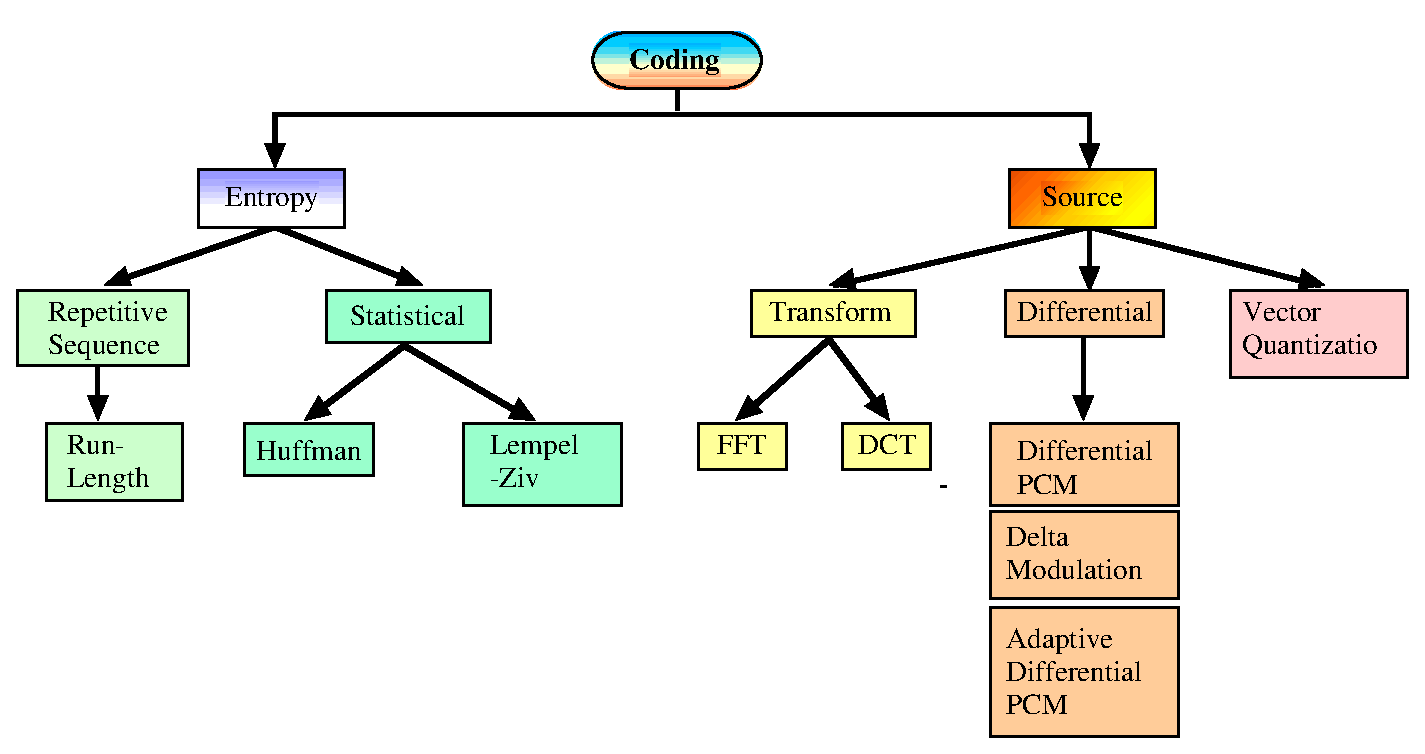
\includegraphics[width=\textwidth]{ch-comp/taxonomy}}
\caption{A taxonomy of coding/compression schemes.\label{fg:taxonomy}}
\end{figure}

So, one scheme for compression is to remove \emph{redundancies} in the
data: that part of the data which conveys no additional information,
given previous data. This is termed \emph{lossless compression},
\index{compression!lossless|emph}
because no information is lost.  Another approach is one which
considers the use to which the data will be put, and selectively
eliminates unneeded or unimportant information --- \emph{lossy
compression}. These two coding schemes and their subcategories are
\index{compression!lossy|emph}
presented in figure~\ref{fg:taxonomy}.  I will discuss many of these
in the rest of this chapter. In each case, I will be concerned with the
following algorithm characteristics:
\begin{itemize}
\item the degree of information loss,
\item the encoding complexity,
\item and the decoding complexity.
\end{itemize}

Why do I separate out encoding and decoding complexity? Isn't decoding
just the opposite of encoding? While that may be true conceptually,
there is no guarantee that, for any particular coding scheme, encoding
and decoding algorithms will have the same run time. Schemes for which
they do are called \emph{symmetric}; those for which they are not are
\emph{asymmetric}.  For some applications, symmetric coding is
necessary, while for others one end (typically the encoder) can be
allowed to take significantly more time (presumably to produce greater
compression or better signal ``quality'' given some level of
compression). In symmetric applications, the hardware and the
available processing time is usually also symmetric, while for
asymmetric applications one end may have much faster hardware and/or
more time.

\begin{figure}
\centerline{\includegraphics[width=\textwidth]{ch-comp/encoding}}
\caption{Generalized scheme for encoding.\label{fg:encoding}}
\end{figure}

So, we arrive at the general scheme for encoding in
figure~\ref{fg:encoding}.  The data to be encoded can first be
transformed (the ``xform'' block) to make it more amenable to
compression (to produce a more compressible representation). The goal
of such a transform is essentially to \emph{expose} the signal's
underlying redundancy. For example, if the signal were a sine wave,
its Fourier transform representation would be more easily
compressible: it would have a single value at one frequency, as
opposed to the original time domain function's sequence of
samples. This representation may also make it easier to separate out
components based on their ``importance'' (allowing more information to
be eliminated from less important components).  I'll discuss this last
point in the sections on lossy compression.

Once the data has been transformed, it is then converted into a
sequence of symbols for transmission. This \emph{quantization} step
\index{compression!quantization and}
limits the number of different symbols to be used.  So, though the
original signal might have 8 bits per sample, it may not be necessary
to retain all 256 symbols. In general, we may map each input symbol to
an output symbol, or we may take $N$ input symbols and produce one
output symbol (this might be the case when ``runs'' of increasing
inputs are common --- we might substitute a single symbol or a shorter
sequence for a stereotypical increasing sequence). Companding is one
example of this kind of quantization: more symbols are allocated to
quiet sections of an audio stream, where small amplitude differences
are noticable, and fewer to loud sections, where much larger
differences are needed for changes in volume to be noticable.  This
stream of symbols are then coded to produce a bit stream, which might
represent each symbol with a varying number of bits, for example. So,
first a quick self-test, and then we'll look at each of these blocks
and compression schemes in more detail.

\problemset{
\subsubsection{Self-Test Exercises}

See~\ref{sc:ch8ex} \#\ref{it:ch8ex3}--\ref{it:ch8ex6} for answers.

\begin{enumerate}
\item If a signal is sent in which all samples have the same value,
  what is the information content in bits (ignoring the first sample)?
\item What kind of signal would have maximum information content?
\item Can you give an example of an application which would demand
  symmetric coding?
\item Can you give an example of an application which could allow
  asymmetric coding?
\end{enumerate}}

\section{Entropy (Lossless) Compression}

\index{compression!lossless|(}
Lossless, or entropy, compression ignores the \emph{semantics}
(meaning) of the data. It is based instead purely on the statistics of
the symbols in the data. These statistics can be the frequencies of
different symbols (how often each occurs) or the existence of
certain \emph{sequences} of symbols. In the former case, we have
statistical compression; in the latter, a category for which
repetitive sequence compression is the simplest case.

\subsection{Repetitive Sequence Compression}

When two people are having a telephone conversation, it is common for
there to be pauses when nobody is speaking. In still images, it is not
unusual for large areas to have the same (usually, background)
color. In video, areas that correspond to moving objects change from
one frame to another while other, larger areas don't change.  All of
these situations have the same feature in their raw stream of samples:
long sequences (1D, 2D, or 3D) which are identical. Many bits are used
to send a relatively small amount of information.

The idea of \emph{run-length encoding} (RLE) is simple: replace long
\index{compression!run-length}
sequences (\emph{runs}) of identical samples with a special code that
indicates the value to be repeated and the number of times to repeat
it. For 8 bits/sample data, we might reserve one symbol (say, zero) as
a ``flag'' to indicate the start of a run length code. A run would
then be replaced with a zero, a byte containing the symbol to repeat
(1--255), and one or more bytes as the repetition count (how many
bytes to use we would have to decide ahead of time, based on what we
know about typical run lengths for the particular kind of signals
being processed). So, for example, a run of 112 `A's in a text file
could be encoded as: \textit{flag}, `A', 112.

We can also extend RLE to work for cases where sequences of symbols,
rather than just one, are repeated.

\subsection{Statistical Compression}

Statistical compression schemes work by assigning
\emph{variable-length codes} to symbols based on their frequency of
occurrence.  By assigning shorter codes to more frequently occurring
symbols, the average number of bits per symbol can be reduced.

\subsubsection{Huffman Coding}

\index{Huffman coding|(}
\index{compression!Huffman|(}
When we sample data, we almost always do so with a fixed number of
bits per sample --- a fixed number of bits per symbol. So, we can
consider 8-bit sampling as quantization of a signal into 256 levels,
or equivalently as representing it as a sequence of symbols, where
there are 256 symbols available.

This is usually \emph{not} the most space-efficient coding scheme, for
the simple reason that some symbols are more common than others.  If
instead we use a variable-length representation, and let more common
symbols be encoded in fewer bits, then we can save a considerable
amount of memory.  While it may be the case that, for a particular
type of signal, the statistics of symbol usage are fairly stable
across multiple data sources, let's not make this assumption. Thus, we
would expect to use the sampled signal itself as the source of
statistical information for code construction.

A \emph{Huffman code} is a variable-length symbol representation
scheme which is optimal in the case where all symbol probabilities are
integral powers of 1/2. Since the number of bits per symbol is
variable, in general the boundary between codes will \emph{not} fall
on byte boundaries. So, there is no ``built in'' demarcation between
symbols.  We could add a special ``marker,'' but this would waste
space.  Rather than waste space, a set of codes with a \emph{prefix
property} is generated: each symbol is encoded into a sequence of bits
so that no code for a symbol is the prefix of the code for any
other. This property allows us to decode a bit string by repeatedly
deleting prefixes of the string that are codes for symbols.  This
prefix property can be assured using binary trees.

\begin{table}[h]
\caption{Two binary codes.\label{tb:prefix}}
\begin{center}
\begin{tabular}{|c|l|l|l|}\hline
\bf Symbol & \bf Probability & \bf Code 1 & \bf Code 2 \\ \hline\hline
a & 0.12 & 000 & 000 \\
b & 0.35 & 001 & 10 \\
c & 0.20 & 010 & 01 \\
d & 0.08 & 011 & 001 \\
e & 0.25 & 100 & 11 \\ \hline
\end{tabular}
\end{center}
\end{table}

Two example codes with the prefix property are given in
Table~\ref{tb:prefix}. Decoding code 1 is easy, as we can just read
three bits at a time (for example, decode ``001010011'' [answer
in~\ref{sc:ch8ex}
\#\ref{it:ch8ex7}]).  For code 2, we must read a bit at a time so
that, for instance, ``1101001'' would be read as ``11''=`2',
``01''=`3', and ``001''=`4'. (What would the symbol sequence be for
``01000001000'' [answer in~\ref{sc:ch8ex}
\#\ref{it:ch8ex8}]?)  Clearly, the
average number of bits per symbol is less for code 2 (2.2 versus 3,
for a saving of 27\%).

So, assuming we have a set of symbols and their probabilities, how do
we find a code with the prefix property such that the average length
of a code for a character is a minimum? The answer is the
\emph{Huffman algorithm}. The basic idea is that we select the two
symbols with the the lowest probabilities (in Table~\ref{tb:prefix},
`1' and `4'), and replace them with a ``made up'' symbol (let's call
it $s_1$) with probability equal to the sum of the original two (in
this example, 0.20).  The optimal prefix code for this set is the code
for $s_1$ (to be determined later) with a zero appended for `1' and a
one appended for `4'. This process is repeated, until all symbols
(real or ``made up'') have been merged into one ``super-symbol'' with
probability 1.0.

If you think about this merging of pairs of characters, what we are
doing is constructing a binary tree from the bottom up.  To find the
code for a symbol, we follow the path from the root to the leaf that
corresponds to it.  Along the way, we output a zero every time we
follow a left child link, and a one for each right link (or we could
use ones for right children and zeros for left, as long as we are
consistent).  If only the leaves of the tree are labeled with symbols,
then we are guaranteed that the code will have the prefix property
(since we only encounter one leaf on the path from the root to a
symbol).  An example code tree (for code~2 in table~\ref{tb:prefix})
is in Figure~\ref{fg:code-tree}.

\begin{figure}
\centerline{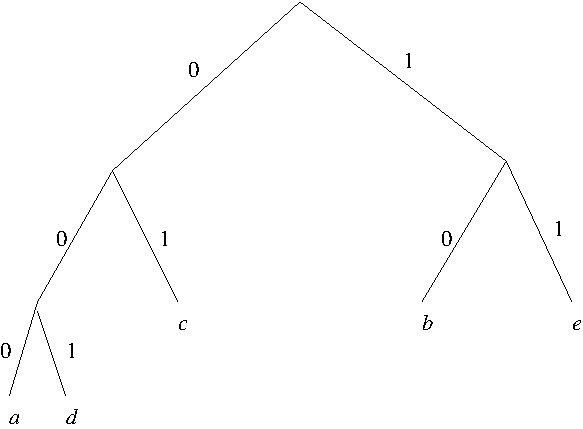
\includegraphics[width=\textwidth]{ch-comp/huffman-tree}}
\caption{Binary tree with prefix property code.\label{fg:code-tree}}
\end{figure}

To compress a signal, then, we build the Huffman tree (there
are more efficient algorithms which don't actually build the tree) and
then produce a \emph{look up table} (like table~\ref{tb:prefix}) that
allows us to generate a code for each symbol (or decode the symbol at
decompression time). We need to send this table with the compressed
signal (or store it in the compressed file).

As I said at the beginning of this section, Huffman coding is only
optimal if the symbol probabilities are integral multiples of 1/2. For
the more general case, \emph{arithmetic coding} can be used.
\index{compression!arithmetic}
\index{arithmetic coding}
\index{compression!Huffman|)}
\index{Huffman coding|)}

\subsubsection{Lempel-Ziv Compression}

In the 1970s, Lempel and Ziv developed two (patented) families of
compression algorithms based on a \emph{dictionary} approach. In a
\index{compression!dictionary based}
nutshell, in one family the algorithm builds a data structure
(dictionary) with entries being sequences of symbols found in the
input data. As the input is scanned, it tries to find the longest
sequence of symbols that already exists in the dictionary.  If this is
successful, the entry number for that dictionary entry is
transmitted.  If unsuccessful, a sequence is added to the dictionary
and also transmitted. This approach starts with sequences of pairs of
symbols and, as the encoding process continues, adds longer and longer
sequences to the dictionary. As a result, long duration signals can be
significantly compressed, as long stretches are found to be repeats of
previously-seen data.
\index{compression!lossless|)}

\section{Source (Lossy) Compression}

\index{compression!lossy|(}
In certain situtations, it may be appropriate to sacrifice some of the
information in the original signal to obtain increased compression.
This may be the case, for instance, when a human observer cannot
perceive the additional information (and therefore won't notice its
lack).  This inability to perceive the difference may be innate to
human perception or it may be a product of the delivery technology
(audio system, video monitor, etc.) or a more subtle interaction of
sampling, the original signal, and human perception (as is the case
for differential compression).
\index{compression!human perception and}

\subsection{Differential Compression}

Recall that when we sample a signal, the discrete representation is
limited to frequencies below the Nyquist cutoff.  It is not uncommon,
however, for a signal to be significantly \emph{oversampled}: the
Nyquist cutoff is much higher than the signal's bandwidth.  Even if
this is not always the case, there may be long stretches of signal for
which it is.  For example, an orchestral recording may have stretches
when no high-pitched instruments are playing.

When a signal lack high-frequency components, this is equivalent to
saying that it changes slowly along time (high frequencies have high
derivatives, low frequencies have small derivatives).  If a signal
changes slowly then, in its sampled version, successive samples are
very similar. Let's go back to the idea of information content being
the part of a message which you don't know.  If we use each sample as
a \emph{prediction} of the next, then the \emph{difference} between
them is the information contained in the second. Ideally, then we
should just transmit this difference.

This is the idea behind \emph{differential pulse code modulation}
(DPCM): we use the $n^\mathrm{th}$ sample of a signal $x[n]$ as the
\index{compression!pulse code modulation (PCM)}
\index{pulse code modulation (PCM)}
\index{differential pulse code modulation}
prediction for the next, $x[n+1]$, and just transmit the difference,
$\Delta x[n+1] = x[n+1] - x[n]3$. Of course, we start our encoding by
sending a complete sample, $x[0]$, and then continue with just the
differences.

In what way is this lossy? It quite possibly isn't, depending on the
number of bits in the original samples, the number of bits in the
differences we send, the possible difference values in the signal, and
how we treat them.  For instance, if our original samples are 8 bits
and we allow 4 bits for differences, we can accommodate differences of
up to $\pm$7 between samples (using a two's complement representation
for the differences).  If all actual differences are less than of
equal to $\pm$7, then no loss results.  What if actual differences are
greater?  We have three basic options:
\begin{enumerate}
\item Output the full sample, rather than just a difference.
\item Assume this is an infrequent anomaly, outputting the maximum
  difference possible and retaining the actual difference internally.
  When subsequent differences are less than the maximum, modify them
  so that the output differences allows the coded signal to ``catch
  up'' to the value of the input.
\item Use the limited number of bits to cover larger differences by
  assuming they are multiplied by a constant factor, in effect
  ``re-quantizing'' them. If the factor was a constant value of `2',
  then 4 bits would cover $\pm$14.
\end{enumerate}

The first case is very straightforward, and clearly results in no
losses.  For the second approach, the reconstructed signal is not the
same as the original --- information has been lost. However, the
information is a rare, sudden change in the signal, and if the
reconstructed signal caught up with the original fairly quickly, it is
likely to be unnoticable. The third approach is also lossy, as it is
incapable of representing differences that fall in between the
quantized levels.

At the extreme, we can allocate only one bit per difference: this is
called \emph{delta modulation} (DM).  In this case, we need to
\index{compression!delta modulation}
\index{delta modulation}
interpret a `0' as a -1 difference and a `1` as a +1 difference (we
could multiply these by a constant factor), so a constant input
produces a ``0101010101\ldots'' sequence, rather than a
``0000000000\ldots'' one.  Assuming the sampling rate is high enough,
differences more than $\pm$1 will be rare, and loss will be minimal.

A more general approach to DPCM would be to use something other than
just the value of one sample to predict the next. Thus, the
differences to be sent (if $m$ values were used) would be $\Delta[n+1]
= \mathcal{F}(x[n-m+1], \ldots, x[n])$.  This is the approach that
\emph{adaptive differential pulse code modulation} (ADPCM) uses.  It
\emph{adapts} to the signal, \index{ADPCM} using past experience to
select the quantization levels that will be used to encode
differences.  This means that loud sections and quiet sections can
have different steps between quantization levels.  The international
videoconferencing standards ITU G.726 use ADPCM to encode audio.

\subsection{Transform Compression}

Going back to figure~\ref{fg:encoding}, one thing that an encoding
scheme can do is to transform the original signal into a domain that
allows for better compression. To allow for better compression, a
representation needs to isolate redundancy. For one-dimensional
signals like audio, redundancy is apparent in the \emph{sequence of
samples}.  All of the previous compression schemes are based on this
sequential redundancy. For a signal sampled along time like sound,
\emph{temporal redundancy} is apparent. For a signal that is spatially
\index{compression!temporal redundancy and}
sampled, like an image, there is a (2D) \emph{spatial redundancy}
\index{compression!spatial redundancy and}
(pixels near each other tend to have similar values).  The question
is: is the above noted temporal or spatial domain the domain in which
the signal has its greatest redundancy, or is there some other domain
in which more redundancy would be apparent? As you might guess, there
are situations in which this is the case (for the aproach to be
practical, we just need to make sure that an \emph{inverse transform},
which brings us back to the original signal domain, exists).

One such domain is the frequency domain. Especially in images, a
spectral representation tends to have great apparent redundancy.  In
such a representation, an image is considered to be composed of the
sum of sinusoids (just as for sound) that are functions of space
(instead of time, as for sound).  The ``only'' conceptual jump here
then is the one from 1D signals to 2D signals, which we'll defer to
chapter~\ref{ch:audio-video}. For the time being, let's think of
images as being one-dimensional, like sound, so we can talk about 1D
Fourier transforms.

I previously said that pixels tend to be similar to those nearby.
This is another way of saying that the change in intensity as a
function of space is low --- that low-frequency processes are
involved.  Repetition coding assumes that there is no change, while
DPCM either places a limit on change or quantizes the changes. Rather
than doing these, let's take the Fourier transform of our signal. We
have now decomposed it according to frequency. If mostly low-frequency
processes have produced our signal, then the coefficients for low
frequencies will have higher values than those for high
frequencies: the low frequency components carry most of the
information.

We can now take the obvious approach: match the number of bits in a
representation to the amount of information contained.  In this case,
rather than use the same number of bits for each frequency
coefficient, we assign more bits to the low frequencies and fewer to
the high.  This approach, which in effect codes different frequency
bands separately, is also called \emph{sub-band coding}.

You probably remember that the Fourier transform (and FFT) have both
magnitude and phase.  We can simplify matters if we use a transform
that uses only real arithmetic.  This is one of the motivations behind
using the discrete cosine transform (DCT) instead.  The DCT
\index{discrete cosine transform (DCT)}
coefficients can be expressed as:

\begin{equation}
X[k] = \sum_{n=0}^{N-1} x[n] \cos2\pi n k/N
\end{equation}

We throw away absolute phase information and assume that the signal
has even symmetry, but since we don't care what happens beyond the
bounds of the signal, this is fine.  Loss of relative phase
information is another matter, but after all, this \emph{is} a lossy
compression technique. In chapter~\ref{ch:audio-video}, I will place
these losses in the context of human perception.
\index{compression!lossy|)}

\section{Problems}

For each of the following MATLAB programming assignments, please email
me your .mat file and your ``best'' result (the result that best shows
the operation of your program). For your result, send both the
original and ``reconstituted'' compressed version.

\begin{enumerate}
\item Write a program that performs run-length coding on images (you
  may treat the image as a one-dimensional vector for processing
  purposes, and in fact MATLAB will allow you to treat 2D matrices in
  this fashion).  What percent compression do you get for black and
  white images (like those that might be produced for sending a fax)?
  What percent for color images generated from drawing programs? What
  percent for images from a digital camera? What percent for vectors
  filled with random numbers?
\item Write a program that performs simple, lossy DPCM coding and
  decoding on sampled audio. Test it using audio samples. For samples
  of people speaking, how many bits do you need for the differences
  for the result to be still intelligible? For it to be of quality
  comparable to the original?
\item For the DCPM examples, can you gain any additional compression
  by applying run-length coding to the output of the DPCM coder? Why
  or why not?
\item One way to apply transform coding of a signal is to divide it
  into \emph{non}-overlapping \emph{windows} and transform and code
  each window separately. Using the same audio samples as before,
  apply DCT coding (MATLAB has \verb|DCT| and \verb|IDCT| functions,
  part of the Signal Processing Toolkit. If this toolkit isn't
  available, use the magnitude of the \verb|FFT|). (Hint: keep the
  window size short; maybe 8 or 16 samples.) Do not try to quantize
  the DC (zero frequency) component, but \emph{do} experiment with
  quantizing the high frequency ones. What is the effect with no
  quantization? See how much compression you can get by heavily
  quantizing and/or eliminating high frequency components.
\end{enumerate}

\section{Further Reading}

\begin{itemize}
\item J. Crowcroft, M. Handley, \& I. Wakeman, \textit{Internetworking
    Multimedia}, Morgan Kaufmann, 1999, chapter~4 (\S\ 4.1--4.5).
\item A. Murat Tekalp, \textit{Digital Video Processing}, Prentice
  Hall, 1995, chapters 18, 19, 21.
\item K.R. Rao \& J.J. Hwang, \textit{Techniques \& Standards for
    Image, Video \& Audio Coding}, Prentice Hall, 1996, chapters 4, 5.
\end{itemize}
